\textbf{\underline{\large{3.5: Integral Approximations: Riemann Rectangles and Trapezoidal Sums}}} \par

We have been focusing on anti-derivatives of functions were the equation is known. But let us suppose we need to evaluate an integral where either the function is unknown or cannot be anti-differentiated---such as $\int_{-2}^3 e^{x^2} \, dx$. This is where the concepts that we touched on in the overview of the chapter come into play. If we have some exact $y$-values, we could approximate the area geometrically. This can be done by dividing the area in question into rectangles, and then finding the area of each rectangle. There are three way to draw the rectangles: \par

\begin{center}
    \fbox{\fbox{\begin{minipage}{0.96\textwidth}
        \vspace{11pt}
        \fbox{\begin{minipage}{0.385\textwidth}
            \includegraphics[width = \textwidth]{\graphicsdir Chapter 3 Graphics/3.5-Graphic1.png}
        \end{minipage}} \vspace{22pt} \begin{minipage}{0.59\textwidth}
            \begin{center}
                Left-Hand Rectangles 
            \end{center}
        \end{minipage}
        \begin{minipage}{0.385\textwidth}
            \includegraphics[width = \textwidth]{\graphicsdir Chapter 3 Graphics/3.5-Graphic2.png}
        \end{minipage} \vspace{22pt} \begin{minipage}{0.59\textwidth}
            \begin{center}
                Midpoint Rectangles 
            \end{center}
        \end{minipage}
        \begin{minipage}{0.385\textwidth}
            \includegraphics[width = \textwidth]{\graphicsdir Chapter 3 Graphics/3.5-Graphic3.png}
        \end{minipage} \vspace{22pt} \begin{minipage}{0.59\textwidth}
            \begin{center}
                Right-Hand Rectangles 
            \end{center}
        \end{minipage}
    \end{minipage}}}
\end{center}

\begin{tcolorbox}[objective]
    \begin{center}
        OBJECTIVES \\[11pt]
    \end{center}
    Find Approximations of Integrals Using Different Rectangles. \\
    Use Proper Notation When Dealing with Integral Approximation.
\end{tcolorbox} \vspace{11pt}

\begin{tcolorbox}[example]
    \textbf{Ex 3.5.1: } Use a left hand Riemann sum with four equal sub-intervals to approximate $\int_1^5 f(x) \, dx$ given the table of values below. \begin{align*}
        \arraycolsep=22pt\def\arraystretch{1.5}
        \begin{array}{|c|c|c|c|c|c|}
            \hline
            x & 1 & 2 & 3 & 4 & 5 \\ \hline
            f(x) & 1 & 4 & 9 & 16 & 25 \\
            \hline
        \end{array}
    \end{align*}
\end{tcolorbox}
\begin{tcolorbox}[solution]
    \textbf{Sol 3.5.1: } Although this problem may seem a little difficult, it's actually quite simple. Let's first recall what a left hand Riemann summation should look like: \\

    \begin{center}
        \includegraphics[width = 0.6\textwidth]{\graphicsdir Chapter 3 Graphics/3.5-Graphic1.png}
    \end{center}
    \vspace{11pt}
    So, to find the areas of the rectangle, we multiply the width of the rectangle by the height. The width of the rectangle is the difference between adjacent $x$-values. Because we are asked to find a left hand Riemann sum, we are gonna start with the leftmost height. Therefore, we have \begin{align*}
        \int_1^5 x^2 \, dx \approx (2 - 1) \cdot 1 + (3 - 2) \cdot 4 + (4 - 3) \cdot 9 + (5 - 4) \cdot 16 = \boxed{30}
    \end{align*}
    Notice how we never use the $f(x)$ value of $25$. This is because when we are using left-hand rectangles, we will never make a rectangle that 
\end{tcolorbox}

With this example, we can create some steps for approximation an integral with rectangles: \par

\textbf{Steps to Approximating an Integral with Rectangles}

\begin{enumerate}
    \item Read the question and determine which type of rectangles to calculate
    \item Write out the integral as a sum of lengths times widths.
    \item Calculate the areas of each rectangle.
    \item Add the areas together for your approximation.
    \item State answer using proper notation.
\end{enumerate}

Although \textbf{Ex 3.5.1} had rectangles of equal width, this does not necessarily have to be true

\begin{tcolorbox}[example]
    \textbf{Ex 3.5.2: } Use a right hand Riemann sum with the sub-intervals defined below to approximate $\int_2^{14} f(x) \, dx$ given the table of values below. \begin{align*}
        \arraycolsep=22pt\def\arraystretch{1.5}
        \begin{array}{|c|c|c|c|c|}
            \hline
            x & 2 & 5 & 10 & 14 \\ \hline
            f(x) & 4 & 10 & 7 & 12 \\
            \hline
        \end{array}
    \end{align*}
\end{tcolorbox}
\begin{tcolorbox}[solution]
    \textbf{Sol 3.5.2: } Let's remind ourselves what a right-hand rectangle approximation looks like: \\

    \begin{center}
        \includegraphics[width = 0.6\textwidth]{\graphicsdir Chapter 3 Graphics/3.5-Graphic3.png}
    \end{center}
    \vspace{11pt}
    Now, as this time we are asked to find a right hand Riemann sum, we start from the right. So, we have \begin{align*}
        \int_2^{14} f(x) \, dx \approx (14 - 10) \cdot 12 + (10 - 5) \cdot 7 + (5 - 2) \cdot 10 = \boxed{113}
    \end{align*}
\end{tcolorbox} 

The third kind of Riemann rectangle is where the height comes from the midpoints of the rectangles. Two conditions are needed for midpoint rectangles: 

\begin{enumerate}
    \item There needs to be an odd number of $x$ values.
    \item The even-numbered (i.e. 2nd, 4th) $x$-values must be midpoints of adjacent $x-values$.
\end{enumerate}

\begin{tcolorbox}[example]
    \textbf{Ex 3.5.3: } The rate of consumption, in gallons per minute, recorded during an airplane flight is given by a twice differentiable and strictly increasing function $R(t)$. A table of selected values for $R(t)$ for the time interval $0 \leq t \leq 90$ is shown below. \begin{align*}
        \arraycolsep=11pt\def\arraystretch{1.5}
        \begin{array}{|c|c|c|c|c|c|c|c|}
            \hline
            t \text{ (minutes)} & 0 & 20 & 40 & 50 & 60 & 90 & 120 \\ \hline
            R(t) \text{ (gallons per minute)} & 20 & 30 & 40 & 55 & 65 & 70 & 95 \\
            \hline
        \end{array}
    \end{align*}
    Use the Riemann sum with midpoint rectangles and the sub-intervals given by the table to approximate the value of $\int_0^{120} R(t) \, dt \forcespace$.
\end{tcolorbox}
\begin{tcolorbox}[solution]
    \textbf{Sol 3.5.3: } Recall the structure of midpoint rectangles: \\
    
    \begin{center}
        \includegraphics[width = 0.6\textwidth]{\graphicsdir Chapter 3 Graphics/3.5-Graphic2.png}
    \end{center}
    \vspace{11pt}
    To find the Riemann sum with midpoint rectangles, we need to take the difference between the odd-numbered $x$-values as our width, and use the $R(t)$ values in between those $x$-values as our height. Therefore, we get \begin{align*}
        \int_0^{120} R(t) \approx (40 - 0) \cdot 30 + (60 - 40) \cdot 55 + (120 - 60) \cdot 70 = \boxed{6500}
    \end{align*}
\end{tcolorbox} \vspace{11pt}

\begin{tcolorbox}[example]
    \textbf{Ex 3.5.4: } Use the midpoint rule and the given data to approximate the value of $\int_0^{2.6} f(x) \, dx$. \begin{align*}
        \arraycolsep=16.5pt\def\arraystretch{1.5}
        \begin{array}{|c|c|c|c|c|c|c|c|}
            \hline
            x & 0 & 0.4 & 0.8 & 1.2 & 1.6 & 2.1 & 2.6 \\ \hline
            f(x) & 3.5 & 2.3 & 3.2 & 4.3 & 4.7 & 5.9 & 4.1 \\
            \hline
        \end{array}
    \end{align*}
\end{tcolorbox} 
\begin{tcolorbox}[solution]
    \textbf{Sol 3.5.4: } For this example, we simply follow the steps in \textbf{Ex 3.5.3}. This gives us \begin{align*}
        \int_0^{2.6} f(x) \, dx \approx (0.8 - 0) \cdot 2.3 + (1.6 - 0.8) \cdot 4.3 + (2.6 - 1.6) \cdot 5.9 = \boxed{11.18}
    \end{align*}
\end{tcolorbox}

The left, right, and midpoint rectangle methods estimate the area under a curve by using rectangles with constant heights. The trapezoidal rule builds on this idea by connecting the tops of the rectangles with straight lines, creating shapes that better match the curve. It can be seen as the average of the left and right rectangle methods and serves as a simple step toward more accurate ways to approximate areas. \par

\begin{tcolorbox}[example]
    \textbf{Ex 3.5.5: } Using the table of data from \textbf{Ex 3.5.4} approximate $\int_0^{2.6} f(x) \, dx$ with 6 trapezoids.
\end{tcolorbox}
\begin{tcolorbox}[solution]
    \textbf{Sol 3.5.5: } Since this is a new method that we are approaching, let's try visualizing it. We can first start by drawing the heights. \\

    \begin{center}
        \includegraphics[width = 0.6\textwidth]{\graphicsdir Chapter 3 Graphics/3.5-Graphic4.png}
    \end{center}
    \vspace{11pt}
    Next, we are gonna connect the points to draw out our trapezoids. \\

    \begin{center}
        \includegraphics[width = 0.6\textwidth]{\graphicsdir Chapter 3 Graphics/3.5-Graphic5.png}
    \end{center}
    \vspace{11pt}
    Now, it becomes pretty clear how we can find the Riemann sum with this method. We use the difference between adjacent $x$-values as the height of the trapezoid, and adjacent pairs of $f(x)$-values as the two bases of the trapezoid. Therefore, let's use the area formula for a trapezoid, \begin{align*}
        A_{\text{trapezoid}} = \left(\dfrac{b_1 + b_2}{2}\right) \cdot h,
    \end{align*}
    to calculate this Riemann sum: \begin{align*}
        \int_0^{2.6} f(x) \, dx & \approx \dfrac{3.5 + 2.3}{2} \cdot (0.4 - 0) + \dfrac{2.3 + 3.2}{2} \cdot (0.8 - 0.4) + \dfrac{3.2 + 4.3}{2} \cdot (1.2 - 0.8) \\[5.5pt]
        & + \dfrac{4.3 + 4.7}{2} \cdot (1.6 - 1.2) + \dfrac{4.7 + 5.9}{2} \cdot (2.1 - 1.6) + \dfrac{5.9 + 4.1}{2} \cdot (2.6 - 2.1) \\[11pt]
        & = \boxed{8.15}
    \end{align*}
\end{tcolorbox}

However, one may notice that this process is quite cumbersome. We have to do multiple computations involving decimals just to get our answer, and sometimes this could lead to arithmetic errors. Luckily, there is a formula that could simplify this process a lot. However, note that this formula could only apply \textbf{if the heights of the trapezoid are all the same}. So, what exactly is this formula? Well, let's take a look. \par

Let's say we have points $x_0, \, x_1, \, x_2, \ldots, x_n$ and $f(x)$ values $f(x_0), \, f(x_1), \, f(x_2), \ldots, f(x_n)$. We know that we are integrating from $x_0$ to $x_n$, we can call those $a$ and $b$, respectively. Since we know that the height of the trapezoids are the same, we know that the height of each trapezoid is the total sum of the heights divided by the number of trapezoids. Therefore, each trapezoid has a height of \begin{align*}
    \dfrac{b - a}{n}.
\end{align*}
Now, let's start writing out the Riemann sum in its complete form. We do the method as we described in $\textbf{Ex 3.5.5}$, taking adjacent $x-values$ as the heights and adjacent pairs of $f(x)$-values as the bases. Therefore, we get{\small{\begin{align*}
    \int_a^b f(x) \, dx \approx \dfrac{f(x_0) + f(x_1)}{2}\left(\dfrac{b - a}{n}\right) + \dfrac{f(x_1) + f(x_2)}{2}\left(\dfrac{b - a}{n}\right) + \cdots + \dfrac{f(x_{n - 1}) + f(x_n)}{2}\left(\dfrac{b - a}{n}\right).
\end{align*}}}
Factoring out $\dfrac{b - a}{n}$ and simplifying the fraction gives us\begin{align*}
    \int_a^b f(x) \, dx \approx \left(\dfrac{b - a}{n}\right)\left(\dfrac{f(x_0) + f(x_1) + f(x_1) + f(x_2) + \cdots f(x_{n - 1}) + f(x_n)}{2}\right).
\end{align*}
We can simplify this even further to \begin{align*}
    \int_a^b f(x) \, dx \approx \left(\dfrac{b - a}{2n}\right)\left(f(x_0) + 2f(x_1) + 2(fx_2) + \cdots + 2f(x_{n - 1}) + f(x_n)\right).
\end{align*}

This gives us the Trapezoidal Rule for equal sub-intervals. \par

\begin{center}
    \fbox{\fbox{\begin{minipage}{0.96\textwidth}
        \vspace{11pt}
        \begin{center}
            \textbf{The Trapezoidal Rule for Riemann summations}
        \end{center}
        \begin{align*}
            \int_a^b f(x) \, dx \approx \left(\dfrac{b - a}{2n}\right)\left(f(x_0) + 2f(x_1) + 2(fx_2) + \cdots + 2f(x_{n - 1}) + f(x_n)\right). \\
        \end{align*}
    \end{minipage}}}
\end{center}

Let's see this formula in use with an example. \par

\begin{tcolorbox}[example]
    \textbf{Ex 3.5.6: } The following table gives values of a continuous function. Approximate the average value of the function using the Trapezoidal Rule.
    \begin{align*}
        \arraycolsep=11pt\def\arraystretch{1.5}
        \begin{array}{|c|c|c|c|c|c|c|c|}
            \hline
            x & 10 & 20 & 30 & 40 & 50 & 60 & 70 \\ \hline
            f(x) & 3.649 & 4.718 & 6.482 & 9.389 & 14.182 & 22.086 & 35.115 \\
            \hline
        \end{array}
    \end{align*}
\end{tcolorbox}
\begin{tcolorbox}[solution]
    \textbf{Sol 3.5.6: } Note that this question is asking for the \textit{average value} of the function. Therefore, we will have to use our average value formula. \begin{align*} 
        f_{avg} &= \dfrac{1}{b - a}\int_a^b f(x) \, dx \\[11pt]
        & = \dfrac{1}{70 - 10}\int_{10}^{70} f(x) \, dx \\[11pt]
        & \approx \dfrac{1}{70 - 10}\left(\dfrac{70 - 10}{2(6)}\right)\begin{aligned}[t]
            (&3.649 + 2 \cdot 4.718 + 2 \cdot 6.482 + 2 \cdot 9.389 \\[5.5pt]
            & + 2 \cdot 14.182 + 2 \cdot 22.086 + 35.115)
        \end{aligned} \\[11pt]
        & = \boxed{12.707}
    \end{align*} 
\end{tcolorbox}

\bigskip

\textbf{\large{Over and Underestimations}} \par

Now that we've learned about the left, right, midpoint, and trapezoidal Riemann sum methods, it's time to explore how these approximations can overestimate or underestimate the true value of an integral. Depending on whether the function is increasing or decreasing, the rectangles or trapezoids we draw may cover too much or too little area under the curve. First, though, let's recall what we know about tangent line approximations: \par

\begin{center}
    \fbox{\fbox{\begin{minipage}{0.96\textwidth}
        \begin{tabbing}
            $\rightarrow$ \= Your approximation will be an \textbf{overestimate} if the curve is \textbf{concave down} (since \\
            \> your ``tangent lines'' will be above the curve). \\[11pt]
            $\rightarrow$ \= Your approximation will be an \textbf{underestimate} if the curve is \textbf{concave up} (since \\
            \> your ``tangent lines'' will be below the curve).
        \end{tabbing}
    \end{minipage}}}
\end{center}

Let's extend that concept to Riemann sums with the following statements. \par

\begin{center}
    \fbox{\fbox{\begin{minipage}{0.96 \textwidth}
        \begin{tabbing}
            $\rightarrow$ \= Left-hand rectangles are an \textbf{overestimate} if the curve is \textbf{decreasing} and an \\
            \> \textbf{underestimate} if the curve is \textbf{increasing}. \\[11pt]
            $\rightarrow$ \= Right-hand rectangles are in \textbf{overestimate} if the curve is \textbf{increasing} and an \\
            \> \textbf{underestimate} if the curve is \textbf{decreasing}. \\[11pt]
            $\rightarrow$ \= Midpoint Rectangles are an \textbf{overestimate} if the curve is \textbf{concave down} and an \\
            \> \textbf{underestimate} if the curve is \textbf{concave down}. \\[11pt]
            $\rightarrow$ \= Trapezoids are an \textbf{overestimate} if the curve is \textbf{concave up} and an \textbf{underestimate} \\
            \> if the curve is \textbf{concave down}.
        \end{tabbing}
    \end{minipage}}}
\end{center}

We can further illustrate this concept with the table in the following page: \par

\hypertarget{chart for over and underestimations}{}
\begin{align*}
    \def\arraystretch{1.5}
    \begin{array}{|c|c|c|}
        \hline
        & \textbf{Decreasing} & \textbf{Increasing} \\
        \hline
        \hspace{5.5pt}\raisebox{-.5\height}{\makebox[0pt][c]{\rotatebox{90}{\textbf{Left Hand}}}}\hspace{5.5pt} &
        \parbox{0.45\textwidth}{\centering
            \vspace{5.5pt}
            \includegraphics[width=0.2\textwidth]{\graphicsdir Chapter 3 Graphics/3.5-Graphic8.png} \\[5.5pt]
            \textit{Overestimate}
            \vspace{5.5pt}
        } &
        \parbox{0.45\textwidth}{\centering
            \vspace{5.5pt}
            \includegraphics[width=0.2\textwidth]{\graphicsdir Chapter 3 Graphics/3.5-Graphic7.png} \\[5.5pt]
            \textit{Underestimate}
            \vspace{5.5pt}
        } \\
        \hline
        \hspace{5.5pt}\raisebox{-.5\height}{\makebox[0pt][c]{\rotatebox{90}{\textbf{Right Hand}}}}\hspace{5.5pt} &
        \parbox{0.45\textwidth}{\centering
            \vspace{5.5pt}
            \includegraphics[width=0.2\textwidth]{\graphicsdir Chapter 3 Graphics/3.5-Graphic9.png} \\[5.5pt]
            \textit{Underestimate}
            \vspace{5.5pt}
        } &
        \parbox{0.45\textwidth}{\centering
            \vspace{5.5pt}
            \includegraphics[width=0.2\textwidth]{\graphicsdir Chapter 3 Graphics/3.5-Graphic6.png} \\[5.5pt]
            \textit{Overestimate}
            \vspace{5.5pt}
        } \\
        \hline
        & \textbf{Concave Up} & \textbf{Concave Down} \\
        \hline
        \hspace{5.5pt}\raisebox{-.5\height}{\makebox[0pt][c]{\rotatebox{90}{\textbf{Trapezoid}}}}\hspace{5.5pt} &
        \parbox{0.45\textwidth}{\centering
            \vspace{5.5pt}
            \includegraphics[width=0.2\textwidth]{\graphicsdir Chapter 3 Graphics/3.5-Graphic10.png} \\[5.5pt]
            \textit{Overestimate}
            \vspace{5.5pt}
        } &
        \parbox{0.45\textwidth}{\centering
            \vspace{5.5pt}
            \includegraphics[width=0.2\textwidth]{\graphicsdir Chapter 3 Graphics/3.5-Graphic11.png} \\[5.5pt]
            \textit{Underestimate}
            \vspace{5.5pt}
        } \\
        \hline
        \hspace{5.5pt}\raisebox{-.5\height}{\makebox[0pt][c]{\rotatebox{90}{\textbf{Midpoint}}}}\hspace{5.5pt} &
        \parbox{0.45\textwidth}{\centering
            \vspace{5.5pt}
            \includegraphics[width=0.2\textwidth]{\graphicsdir Chapter 3 Graphics/3.5-Graphic12.png} \\[5.5pt]
            \textit{Underestimate}
            \vspace{5.5pt}
        } &
        \parbox{0.45\textwidth}{\centering
            \vspace{5.5pt}
            \includegraphics[width=0.2\textwidth]{\graphicsdir Chapter 3 Graphics/3.5-Graphic13.png} \\[5.5pt]
            \textit{Overestimate}
            \vspace{5.5pt}
        } \\
        \hline
    \end{array}
\end{align*}

\newpage

\textbf{\large{3.5 Free Response Homework}} \par

\onequestion{1. The following table gives values of a continuous function:} \begin{align*}
    \arraycolsep=16.5pt\def\arraystretch{1.5}
    \begin{array}{|c|c|c|c|c|c|c|c|c|c|}
        \hline
        x & 0 & 1 & 2 & 3 & 4 & 5 & 6 & 7 & 8\\ \hline
        F(x) & 10 & 15 & 17 & 12 & 3 & -5 & 8 & -2 & 10 \\
        \hline
    \end{array}
\end{align*}

Estimate the average value of the function on $x \in [0, \, 8]$ using: 
\begin{enumerate}[label=\hspace{11pt}(\alph*), align=left, leftmargin=*, labelsep=0.25em]
    \item right-hand Riemann rectangles.
    \item left-hand Riemann rectangles.
    \item midpoint Riemann rectangles.
\end{enumerate} \vspace{11pt}

\onequestion{2. The velocity of a car was read from its speedometer at 10-second intervals and recorded in the table. Use the midpoint rule to estimate the distance traveled by the car.} \begin{align*}
    \arraycolsep=16.5pt\def\arraystretch{1.5}
    \begin{array}{|c|c|c|c|c|c|c|}
        \hline
        t \text{ (seconds)} & 0 & 10 & 20 & 30 & 40 & 50 \\ \hline
        v(t) \text{ (mi/h)} & 0 & 38 & 52 & 58 & 55 & 51 \\ \hline
        t \text{ (seconds)} & 60 & 70 & 80 & 90 & 100 & \cellcolor{gray!70}\\ \hline
        v(t) \text{ (mi/h)} & 56 & 53 & 50 & 47 & 45 & \cellcolor{gray!70} \\ 
        \hline
    \end{array}
\end{align*} 

\onequestion{3. Below is a chart showing the rate of a rocket flying according to time in minutes:} \begin{align*}
    \arraycolsep=16.5pt\def\arraystretch{1.5}
    \begin{array}{|c|c|c|c|c|c|c|c|}
        \hline
        t \text{ (minutes)} & 0 & 10 & 20 & 30 & 40 & 50 & 60 \\ \hline
        v(t) \text{ (km/h)} & 30 & 28 & 32 & 18 & 52 & 48 & 28 \\
        \hline
    \end{array}
\end{align*}

Use this information to answer each of the questions below. Make sure you express your answer in correct units. 
\begin{enumerate}[label=\hspace{11pt}(\alph*), align=left, leftmargin=*, labelsep=0.25em]
    \item Find an approximation for $\int_0^{60} v(t) \, dt$ using midpoint rectangles. 
    \item Find an approximation for $\int_0^{30} v(t) \, dt$ using trapezoids. 
    \item Find an approximation for $\int_{30}^{60} v(t) \, dt$ using left-hand rectangles.
    \item Find an approximation for $\int_{0}^{40} v(t) \, dt$ using right-hand rectangles.
\end{enumerate} \vspace{11pt}

\onequestion{4. Below is a chart showing the rate of water flowing through a pipeline according to time in minutes:} \begin{align*}
    \arraycolsep=16.5pt\def\arraystretch{1.5}
    \begin{array}{|c|c|c|c|c|c|c|c|}
        \hline
        t \text{ (minutes)} & 0 & 8 & 16 & 24 & 32 & 40 & 48 \\ \hline
        V(t) \si{(m^3 \per min)} & 26 & 32 & 43 & 24 & 19 & 24 & 26 \\
        \hline
    \end{array}
\end{align*}

Use this information to answer each of the questions below. Make sure you express your answer in correct units.
\begin{enumerate}[label=\hspace{11pt}(\alph*), align=left, leftmargin=*, labelsep=0.25em]
    \item Find an approximation for $\int_0^{48} V(t) \, dt$ using midpoint rectangles. 
    \item Find an approximation for $\int_0^{16} V(t) \, dt$ using right-hand rectangles. 
\end{enumerate} \vspace{11pt}

\onequestion{5. Below is a chart of your speed driving to school in meters per second:} \begin{align*}
    \arraycolsep=16.5pt\def\arraystretch{1.5}
    \begin{array}{|c|c|c|c|c|c|c|c|}
        \hline
        t \text{ (seconds)} & 0 & 30 & 90 & 120 & 220 & 300 & 360 \\ \hline
        v(t) \text{ (m/sec)} & 0 & 21 & 43 & 38 & 30 & 24 & 0 \\
        \hline
    \end{array}
\end{align*}

Use this information to answer each of the questions below. Make sure you express your answer in correct units.
\begin{enumerate}[label=\hspace{11pt}(\alph*), align=left, leftmargin=*, labelsep=0.25em]
    \item Find an approximation for $\int_0^{360} v(t) \, dt$ using left-hand rectangles. 
    \item Find an approximation for $\int_0^{220} v(t) \, dt$ using trapezoids. 
\end{enumerate} \vspace{11pt}

\onequestion{6. Below is a chart showing the velocity of the Flash is he runs across the country:} \begin{align*}
    \arraycolsep=16.5pt\def\arraystretch{1.5}
    \begin{array}{|c|c|c|c|c|c|c|c|}
        \hline
        t \text{ (seconds)} & 0 & 4 & 8 & 12 & 16 & 20 & 24 \\ \hline
        v(t) \text{ (km/sec)} & 10 & 12 & 15 & 19 & 24 & 18 & 7 \\
        \hline
    \end{array}
\end{align*}

Use this information to answer each of the questions below. Make sure you express your answer in correct units.
\begin{enumerate}[label=\hspace{11pt}(\alph*), align=left, leftmargin=*, labelsep=0.25em]
    \item Find an approximation for $\int_0^{24} v(t) \, dt$ using midpoint rectangles. 
    \item Find an approximation for $\int_0^{16} v(t) \, dt$ using trapezoids. 
\end{enumerate} \vspace{11pt}

\onequestion{7. Below is a chart showing the rate of sewage flowing through a pipeline according to time in minutes:} \begin{align*}
    \arraycolsep=16.5pt\def\arraystretch{1.5}
    \begin{array}{|c|c|c|c|c|c|c|c|}
        \hline
        t \text{ (minutes)} & 0 & 4 & 6 & 10 & 13 & 15 & 20 \\ \hline
        V(t) \text{ (gallons/min)} & 83 & 68 & 82 & 40 & 38 & 30 & 68 \\
        \hline
    \end{array}
\end{align*}

Use this information to answer each of the questions below. Make sure you express your answer in correct units.
\begin{enumerate}[label=\hspace{11pt}(\alph*), align=left, leftmargin=*, labelsep=0.25em]
    \item Find an approximation for $\int_0^{20} V(t) \, dt$ using trapezoids. 
    \item Find an approximation for $\int_0^{20} V(t) \, dt$ using left-hand rectangles. 
\end{enumerate} \vspace{11pt}

\onequestion{8. Star Formation Rate (SFR) observations of red-shift allow scientists to track the total mass gained in a galaxy by the making of new stars. Below is a table of such data:} \begin{align*}
    \arraycolsep=5.5pt\def\arraystretch{1.5}
    \begin{array}{|c|c|c|c|c|c|c|c|c|c|}
        \hline
        t & 0 & 1 & 2 & 3 & 4 & 5 & 6 & 7 & 8 \\ \hline
        \text{SFR} & 0.0029 & 0.0051 & 0.0055 & 0.0049 & 0.0042 & 0.0035 & 0.0029 & 0.0025 & 0.0021 \\
        \hline
    \end{array}
\end{align*}

SFR is measured in solar masses per cubic parsec per gigayear (millions of years), and $t$ is measured in gigayears. 
\begin{enumerate}[label=\hspace{11pt}(\alph*), align=left, leftmargin=*, labelsep=0.25em]
    \item Use midpoint rectangles to approximate the total mass of stars formed from $t = 0$ to $t = 8$.
    \item Use right-hand rectangles to approximate the average solar masses per cubic parsec per gigayear.
\end{enumerate} \vspace{11pt}

\onequestion{9. Use (a) the trapezoidal rule and (b) the midpoint rule to approximate $\int_0^2 \sqrt[4]{1 + x^2} \, dx$ with the specified value of $n = 8$ (8 intervals).} \\[11pt]
\onequestion{10. Use (a) the trapezoidal rule and (b) the midpoint rule to approximate $\int_1^2 \dfrac{\ln x}{1 + x} \, dx$ with the specified value of $n = 10$ (10 intervals).} \\[11pt]

\textbf{\large{3.5 Multiple Choice Homework}} \par
\begin{questions}
    \question The graph of the function $f$ is shown below for $0 \leq x \leq 3$. \begin{align*}
        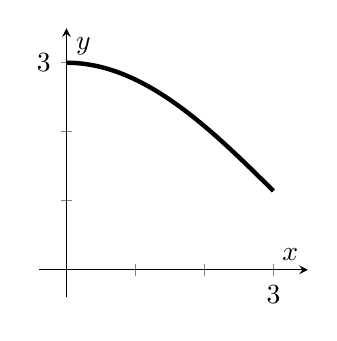
\begin{tikzpicture}
            \begin{axis}[
                axis lines = middle,
                xlabel = $x$,
                ylabel = $y$,
                domain = 0:3,
                samples = 100,
                width=5cm,
                height=5cm,
                xmin = -0.4, xmax = 3.5,
                xtick = {1, 2, 3},
                xticklabels = {, ,$3$},
                ymin = -0.4, ymax = 3.5,
                ytick = {1, 2, 3},
                yticklabels = {, , $3$}
            ]
              \addplot[ultra thick] {2 * cos(deg(x / 2)) + 1};
            \end{axis}
        \end{tikzpicture}
    \end{align*}
    Of the following, which has the smallest value? Assume each approximation is done with $6$ equal subintervals. \\

    \begin{oneparchoices}
        \choice $\int_1^3 f(x) \, dx$ \\[11pt]
        \makebox[0.035\textwidth] \choice Left-hand Riemann approximation of $\int_1^3 f(x) \, dx$. \\[11pt]
        \makebox[0.035\textwidth] \choice Right-hand Riemann approximation of $\int_1^3 f(x) \, dx$. \\[11pt]
        \makebox[0.035\textwidth] \choice Midpoint Riemann approximation of $\int_1^3 f(x) \, dx$. \\[11pt]
        \makebox[0.035\textwidth] \choice Trapezoidal approximation of $\int_1^3 f(x) \, dx$.
    \end{oneparchoices} \par \horizontalline

    \question The table below gives the values for the rate at which water flowed into a lake, with readings taken at specific times. \begin{align*}
        \arraycolsep=16.5pt\def\arraystretch{1.5}
        \begin{array}{|c|c|c|c|c|c|c|}
            \hline
            \text{Time (sec)} & 0 & 10 & 25 & 37 & 46 & 60 \\ \hline
            \text{Rate (gal/sec)} & 500 & 400 & 350 & 280 & 200 & 180 \\
            \hline
        \end{array}
    \end{align*}
    A right-hand Riemann sum, with the five subintervals indicated by the data in the table, is used to estimate the total amount of water that flowed into the lake during the time period $0 \leq t \leq 60$. What is this estimate? \\

    \begin{oneparchoices}
        \choice $1910 \si{gal}$
        \choice $14100 \si{gal}$
        \choice $16930 \si{gal}$
        \choice $18725 \si{gal}$
        \choice $20520 \si{gal}$
    \end{oneparchoices} \par \horizontalline

    \question A car is traveling on a straight road such that selected measures of the velocity have values given on the table below. \begin{align*}
        \arraycolsep=22pt\def\arraystretch{1.5}
        \begin{array}{|c|c|c|c|c|c|}
            \hline
            t \text{ (sec)} & 10 & 20 & 40 & 70 & 80 \\ \hline
            v(t) \text{ (m/sec)} & 90 & 88 & 100 & 90 & 85 \\
            \hline
        \end{array}
    \end{align*}
    Using four left-hand Riemann rectangles based on this table, the estimated distance traveled by the car between $t = 10$ and $t = 80$ seconds is \\

    \begin{oneparchoices}
        \choice $6125 \si{m}$
        \choice $6380 \si{m}$
        \choice $6430 \si{m}$
        \choice $6495 \si{m}$
        \choice $6560 \si{m}$
    \end{oneparchoices} \par \horizontalline

    \question The function $f$, with some values represented in the table below, is continuous and differentiable on the closed interval $[3, \, 12]$. \begin{align*}
        \arraycolsep=22pt\def\arraystretch{1.5}
        \begin{array}{|c|c|c|c|c|c|}
            \hline
            x & 3 & 6 & 9 & 12 \\ \hline
            f(x) & 12 & 8 & 7 & 5 \\
            \hline
        \end{array}
    \end{align*}
    What is the right Riemann approximation of $\int_3^{12} f(x) \, dx$? \\

    \begin{oneparchoices}
        \choice $69$
        \choice $90$
        \choice $111$
        \choice $126$
        \choice $201$
    \end{oneparchoices}  \par \horizontalline

    \question Consider the function $f$ whose graph is shown below: 
    \begin{center}
        \includegraphics[width = 0.55\textwidth]{\graphicsdir Chapter 3 Graphics/3.5-Graphic14.png}
    \end{center}
    The approximate value of $\int_0^8 f(x) \, dx$, using eight right-hand rectangles with equal widths is \\

    \begin{oneparchoices}
        \choice $18.5$
        \choice $37$
        \choice $40$
        \choice $40.5$
        \choice $44$
    \end{oneparchoices} \par \horizontalline

    \question Consider the function $f$ whose graph is shown below: 
    \begin{center}
        \includegraphics[width = 0.55\textwidth]{\graphicsdir Chapter 3 Graphics/3.5-Graphic14.png}
    \end{center}
    The approximate value of $\int_0^8 f(x) \, dx$, using eight left-hand rectangles with equal widths, is \\

    \begin{oneparchoices}
        \choice $23$
        \choice $37$
        \choice $40$
        \choice $40.5$
        \choice $44$
    \end{oneparchoices} \par \horizontalline

    \question Consider the function $f$ whose graph is shown below: 
    \begin{center}
        \includegraphics[width = 0.55\textwidth]{\graphicsdir Chapter 3 Graphics/3.5-Graphic14.png}
    \end{center}
    The approximate value of $\int_0^8 f(x) \, dx$, using eight trapezoids with equal widths, is \\

    \begin{oneparchoices}
        \choice $37$
        \choice $40$
        \choice $40.5$
        \choice $44$
        \choice $48$
    \end{oneparchoices} \par \horizontalline

    \question Consider the function $f$ whose graph is shown below: 
    \begin{center}
        \includegraphics[width = 0.55\textwidth]{\graphicsdir Chapter 3 Graphics/3.5-Graphic14.png}
    \end{center}
    The approximate value of $\int_0^8 f(x) \, dx$, using four midpoint rectangles with equal widths, is \\

    \begin{oneparchoices}
        \choice $20$
        \choice $37$
        \choice $40$
        \choice $40.5$
        \choice $44$
    \end{oneparchoices} \par \horizontalline

    \question Let $f$ be a differentiable function on the closed interval $[2, \, 14]$ and which has values shown on the table below. \begin{align*}
        \arraycolsep=22pt\def\arraystretch{1.5}
        \begin{array}{|c|c|c|c|c|c|}
            \hline
            x & 2 & 5 & 10 & 14 \\ \hline
            f(x) & 12 & 28 & 34 & 30 \\
            \hline
        \end{array}
    \end{align*}
    Using the sub-intervals defined by the table, estimate $\int_2^{14} f(x) \,dx$ using a right-hand Riemann approximation. \\

    \begin{oneparchoices}
        \choice $296$
        \choice $312$
        \choice $343$
        \choice $374$
        \choice $390$
    \end{oneparchoices} \par \horizontalline

    \question The following table lists the known values of a function $f(x)$. \begin{align*}
        \arraycolsep=22pt\def\arraystretch{1.5}
        \begin{array}{|c|c|c|c|c|c|c|}
            \hline
            x & 1 & 2 & 3 & 4 & 5 \\ \hline
            f(x) & 0 & 1.1 & 1.4 & 1.2 & 1.5 \\
            \hline
        \end{array}
    \end{align*}
    Use the trapezoidal rule to approximate $\int_1^5 f(x) \, dx$. \\

    \begin{oneparchoices}
        \choice $4.1$
        \choice $4.3$
        \choice $4.5$
        \choice $4.7$
        \choice $4.9$
    \end{oneparchoices} \par \horizontalline

    \question A small plant is purchased from a nursery and the change in height of the plant is measured at the end of the each day for four days. The data, where $H(t)$ is measured in inches per day and $t$ is measured in days, are listed below. \begin{align*}
        \arraycolsep=22pt\def\arraystretch{1.5}
        \begin{array}{|c|c|c|c|c|c|c|}
            \hline
            x & 0 & 1 & 2 & 3 & 4 \\ \hline
            f(x) & 0 & 1.3 & 1.5 & 2.1 & 2.6 \\
            \hline
        \end{array}
    \end{align*}
    Using the trapezoidal rule, which of the following represents an estimate of the average rate of growth of the plant over the four-day period? \\

    \begin{oneparchoices}
        \choice $\dfrac{1}{4}(0 + 1.3 + 1.5 + 2.1 + 2.6)$ \\[11pt]
        \makebox[0.035\textwidth] \choice $\dfrac{1}{4}\left[\dfrac{1}{2}(0 + 1.3 + 1.5 + 2.1 + 2.6)\right]$ \\[11pt]
        \makebox[0.035\textwidth] \choice $\dfrac{1}{4}\left[\dfrac{1}{2}(0 + 2(1.3) + 2(1.5) + 2(2.1) + 2.6)\right]$ \\[11pt]
        \makebox[0.035\textwidth] \choice $\dfrac{1}{4}\left[\dfrac{1}{2}(0 + 2(1.3) + 2(1.5) + 2(2.1) + 2(2.6))\right]$ \\[11pt]
        \makebox[0.035\textwidth] \choice $\dfrac{1}{4}\left[\dfrac{1}{4}(0 + 2(1.3) + 2(1.5) + 2(2.1) + 2.6)\right]$
    \end{oneparchoices} \par \horizontalline
\end{questions}